% Options for packages loaded elsewhere
\PassOptionsToPackage{unicode}{hyperref}
\PassOptionsToPackage{hyphens}{url}
%
\documentclass[
]{article}
\usepackage{amsmath,amssymb}
\usepackage{iftex}
\ifPDFTeX
  \usepackage[T1]{fontenc}
  \usepackage[utf8]{inputenc}
  \usepackage{textcomp} % provide euro and other symbols
\else % if luatex or xetex
  \usepackage{unicode-math} % this also loads fontspec
  \defaultfontfeatures{Scale=MatchLowercase}
  \defaultfontfeatures[\rmfamily]{Ligatures=TeX,Scale=1}
\fi
\usepackage{lmodern}
\ifPDFTeX\else
  % xetex/luatex font selection
\fi
% Use upquote if available, for straight quotes in verbatim environments
\IfFileExists{upquote.sty}{\usepackage{upquote}}{}
\IfFileExists{microtype.sty}{% use microtype if available
  \usepackage[]{microtype}
  \UseMicrotypeSet[protrusion]{basicmath} % disable protrusion for tt fonts
}{}
\makeatletter
\@ifundefined{KOMAClassName}{% if non-KOMA class
  \IfFileExists{parskip.sty}{%
    \usepackage{parskip}
  }{% else
    \setlength{\parindent}{0pt}
    \setlength{\parskip}{6pt plus 2pt minus 1pt}}
}{% if KOMA class
  \KOMAoptions{parskip=half}}
\makeatother
\usepackage{xcolor}
\usepackage[margin=1in]{geometry}
\usepackage{color}
\usepackage{fancyvrb}
\newcommand{\VerbBar}{|}
\newcommand{\VERB}{\Verb[commandchars=\\\{\}]}
\DefineVerbatimEnvironment{Highlighting}{Verbatim}{commandchars=\\\{\}}
% Add ',fontsize=\small' for more characters per line
\usepackage{framed}
\definecolor{shadecolor}{RGB}{248,248,248}
\newenvironment{Shaded}{\begin{snugshade}}{\end{snugshade}}
\newcommand{\AlertTok}[1]{\textcolor[rgb]{0.94,0.16,0.16}{#1}}
\newcommand{\AnnotationTok}[1]{\textcolor[rgb]{0.56,0.35,0.01}{\textbf{\textit{#1}}}}
\newcommand{\AttributeTok}[1]{\textcolor[rgb]{0.13,0.29,0.53}{#1}}
\newcommand{\BaseNTok}[1]{\textcolor[rgb]{0.00,0.00,0.81}{#1}}
\newcommand{\BuiltInTok}[1]{#1}
\newcommand{\CharTok}[1]{\textcolor[rgb]{0.31,0.60,0.02}{#1}}
\newcommand{\CommentTok}[1]{\textcolor[rgb]{0.56,0.35,0.01}{\textit{#1}}}
\newcommand{\CommentVarTok}[1]{\textcolor[rgb]{0.56,0.35,0.01}{\textbf{\textit{#1}}}}
\newcommand{\ConstantTok}[1]{\textcolor[rgb]{0.56,0.35,0.01}{#1}}
\newcommand{\ControlFlowTok}[1]{\textcolor[rgb]{0.13,0.29,0.53}{\textbf{#1}}}
\newcommand{\DataTypeTok}[1]{\textcolor[rgb]{0.13,0.29,0.53}{#1}}
\newcommand{\DecValTok}[1]{\textcolor[rgb]{0.00,0.00,0.81}{#1}}
\newcommand{\DocumentationTok}[1]{\textcolor[rgb]{0.56,0.35,0.01}{\textbf{\textit{#1}}}}
\newcommand{\ErrorTok}[1]{\textcolor[rgb]{0.64,0.00,0.00}{\textbf{#1}}}
\newcommand{\ExtensionTok}[1]{#1}
\newcommand{\FloatTok}[1]{\textcolor[rgb]{0.00,0.00,0.81}{#1}}
\newcommand{\FunctionTok}[1]{\textcolor[rgb]{0.13,0.29,0.53}{\textbf{#1}}}
\newcommand{\ImportTok}[1]{#1}
\newcommand{\InformationTok}[1]{\textcolor[rgb]{0.56,0.35,0.01}{\textbf{\textit{#1}}}}
\newcommand{\KeywordTok}[1]{\textcolor[rgb]{0.13,0.29,0.53}{\textbf{#1}}}
\newcommand{\NormalTok}[1]{#1}
\newcommand{\OperatorTok}[1]{\textcolor[rgb]{0.81,0.36,0.00}{\textbf{#1}}}
\newcommand{\OtherTok}[1]{\textcolor[rgb]{0.56,0.35,0.01}{#1}}
\newcommand{\PreprocessorTok}[1]{\textcolor[rgb]{0.56,0.35,0.01}{\textit{#1}}}
\newcommand{\RegionMarkerTok}[1]{#1}
\newcommand{\SpecialCharTok}[1]{\textcolor[rgb]{0.81,0.36,0.00}{\textbf{#1}}}
\newcommand{\SpecialStringTok}[1]{\textcolor[rgb]{0.31,0.60,0.02}{#1}}
\newcommand{\StringTok}[1]{\textcolor[rgb]{0.31,0.60,0.02}{#1}}
\newcommand{\VariableTok}[1]{\textcolor[rgb]{0.00,0.00,0.00}{#1}}
\newcommand{\VerbatimStringTok}[1]{\textcolor[rgb]{0.31,0.60,0.02}{#1}}
\newcommand{\WarningTok}[1]{\textcolor[rgb]{0.56,0.35,0.01}{\textbf{\textit{#1}}}}
\usepackage{graphicx}
\makeatletter
\def\maxwidth{\ifdim\Gin@nat@width>\linewidth\linewidth\else\Gin@nat@width\fi}
\def\maxheight{\ifdim\Gin@nat@height>\textheight\textheight\else\Gin@nat@height\fi}
\makeatother
% Scale images if necessary, so that they will not overflow the page
% margins by default, and it is still possible to overwrite the defaults
% using explicit options in \includegraphics[width, height, ...]{}
\setkeys{Gin}{width=\maxwidth,height=\maxheight,keepaspectratio}
% Set default figure placement to htbp
\makeatletter
\def\fps@figure{htbp}
\makeatother
\setlength{\emergencystretch}{3em} % prevent overfull lines
\providecommand{\tightlist}{%
  \setlength{\itemsep}{0pt}\setlength{\parskip}{0pt}}
\setcounter{secnumdepth}{-\maxdimen} % remove section numbering
\usepackage{booktabs, longtable, array, multirow, wrapfig, float, colortbl, pdflscape, tabu, threeparttable, threeparttablex, makecell, xcolor, upgreek}
\usepackage{booktabs}
\usepackage{longtable}
\usepackage{array}
\usepackage{multirow}
\usepackage{wrapfig}
\usepackage{float}
\usepackage{colortbl}
\usepackage{pdflscape}
\usepackage{tabu}
\usepackage{threeparttable}
\usepackage{threeparttablex}
\usepackage[normalem]{ulem}
\usepackage{makecell}
\usepackage{xcolor}
\ifLuaTeX
  \usepackage{selnolig}  % disable illegal ligatures
\fi
\IfFileExists{bookmark.sty}{\usepackage{bookmark}}{\usepackage{hyperref}}
\IfFileExists{xurl.sty}{\usepackage{xurl}}{} % add URL line breaks if available
\urlstyle{same}
\hypersetup{
  pdftitle={Scripted PDF},
  pdfauthor={Tim Bergsma},
  hidelinks,
  pdfcreator={LaTeX via pandoc}}

\title{Scripted PDF}
\author{Tim Bergsma}
\date{2024-11-25}

\begin{document}
\maketitle

The point of this exercise is to demonstrate flexible rendering of
subscripts and superscripts. We want to write expressions for column
labels and units that are fairly readable as they are, and yet can be
easily rendered with equivalent results in plotmath, html, or pdf.

First we load some packages.

\begin{Shaded}
\begin{Highlighting}[]
\FunctionTok{library}\NormalTok{(magrittr)}
\FunctionTok{library}\NormalTok{(ggplot2)}
\FunctionTok{library}\NormalTok{(tablet)}
\FunctionTok{library}\NormalTok{(yamlet)}
\FunctionTok{library}\NormalTok{(dplyr)}
\FunctionTok{library}\NormalTok{(kableExtra)}
\end{Highlighting}
\end{Shaded}

We create some example data.

\begin{Shaded}
\begin{Highlighting}[]
\NormalTok{x }\OtherTok{\textless{}{-}} \FunctionTok{data.frame}\NormalTok{(}
  \AttributeTok{time =} \DecValTok{1}\SpecialCharTok{:}\DecValTok{10}\NormalTok{, }
  \AttributeTok{work =}\NormalTok{ (}\DecValTok{1}\SpecialCharTok{:}\DecValTok{10}\NormalTok{)}\SpecialCharTok{\^{}}\FloatTok{1.5}\NormalTok{, }
  \AttributeTok{group =} \DecValTok{1}\SpecialCharTok{:}\DecValTok{2}\NormalTok{, }
  \AttributeTok{set =} \FunctionTok{c}\NormalTok{(}\FunctionTok{rep}\NormalTok{(}\StringTok{\textquotesingle{}delta\textquotesingle{}}\NormalTok{,}\DecValTok{5}\NormalTok{), }\FunctionTok{rep}\NormalTok{(}\StringTok{\textquotesingle{}gamma\textquotesingle{}}\NormalTok{, }\DecValTok{5}\NormalTok{))}
\NormalTok{)}
\NormalTok{x }\SpecialCharTok{\%\textless{}\textgreater{}\%} \FunctionTok{decorate}\NormalTok{(}\StringTok{\textquotesingle{}}
\StringTok{ time: [ Time\_cum.\^{}alpha, h ]}
\StringTok{ work: [ Work\_total\_obs}\SpecialCharTok{\textbackslash{}\textbackslash{}}\StringTok{n, kg*m\^{}2/s\^{}2 ]}
\StringTok{ group: [ Group, [ Second}\SpecialCharTok{\textbackslash{}\textbackslash{}}\StringTok{nGroup\^{}}\SpecialCharTok{\textbackslash{}\textbackslash{}}\StringTok{*: 2, First}\SpecialCharTok{\textbackslash{}\textbackslash{}}\StringTok{nGroup\^{}\#: 1 ]]}
\StringTok{ set: [ Set, [ gamma, delta ]]}
\StringTok{\textquotesingle{}}\NormalTok{)}
\NormalTok{x }\SpecialCharTok{\%\textgreater{}\%}\NormalTok{ decorations}
\end{Highlighting}
\end{Shaded}

\begin{verbatim}
## - time
##  - label: Time_cum.^alpha
##  - guide: h
## - work
##  - label: Work_total_obs\n
##  - guide: kg*m^2/s^2
## - group
##  - label: Group
##  - guide
##   - Second\nGroup^\*: 2
##   - First\nGroup^#: 1
## - set
##  - label: Set
##  - guide: gamma, delta
\end{verbatim}

The label for column \texttt{work} has nested subscripts suggesting
\(\sf{Work_{total_{obs}}}\). The label for column \texttt{time} suggests
\(\sf{Time_{cum}{}^{\alpha}}\). The dot closes the subscript to
distinguish this from \(\sf{Time_{cum^{\alpha}}}\). Backslash-n requests
a line break.

How does this look when we plot it?

\begin{Shaded}
\begin{Highlighting}[]
\NormalTok{x }\SpecialCharTok{\%\textgreater{}\%} 
\NormalTok{  resolve }\SpecialCharTok{\%\textgreater{}\%} 
  \FunctionTok{ggplot}\NormalTok{(}\FunctionTok{aes}\NormalTok{(time, work, }\AttributeTok{color =}\NormalTok{ group, }\AttributeTok{shape =}\NormalTok{ set)) }\SpecialCharTok{+} 
  \FunctionTok{geom\_point}\NormalTok{()}
\end{Highlighting}
\end{Shaded}

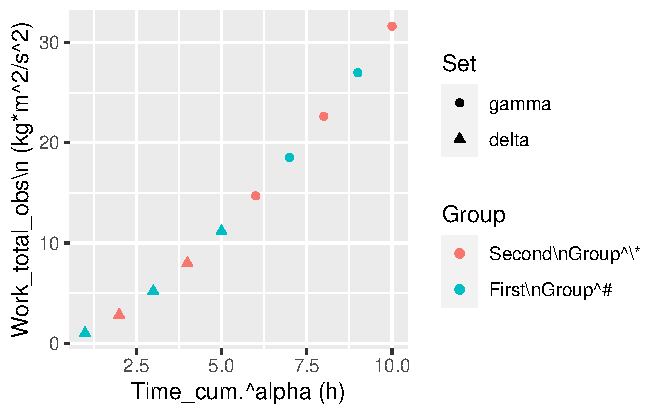
\includegraphics[width=0.5\linewidth]{C:/project/devel/yamlet/vignettes/scripted-pdf_files/figure-latex/unnamed-chunk-4-1}

By default, we get verbatim labels and units as substitutes for column
names.

Next, we use \texttt{enscript()} instead of \texttt{resolve()} to
indicate that the labels should be understood as potentially having
subscripts and superscripts. For this to work well, units should be
constructed using *, /, and \^{} (even though the ``units'' package
supports other encodings).

\begin{Shaded}
\begin{Highlighting}[]
\NormalTok{x }\SpecialCharTok{\%\textgreater{}\%} 
\NormalTok{  enscript }\SpecialCharTok{\%\textgreater{}\%} 
  \FunctionTok{ggplot}\NormalTok{(}\FunctionTok{aes}\NormalTok{(time, work, }\AttributeTok{color =}\NormalTok{ group, }\AttributeTok{shape =}\NormalTok{ set)) }\SpecialCharTok{+} 
  \FunctionTok{geom\_point}\NormalTok{()}
\end{Highlighting}
\end{Shaded}

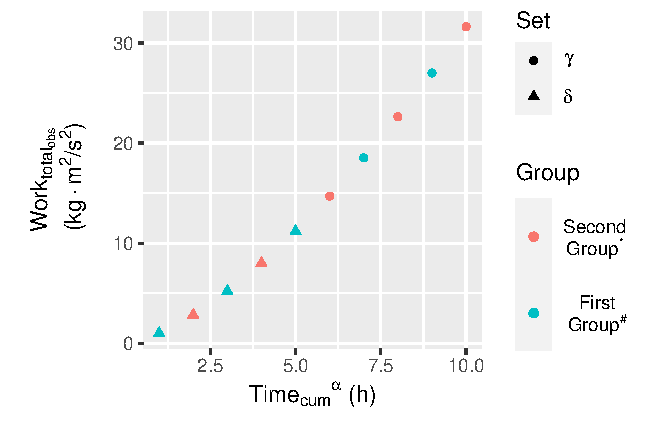
\includegraphics[width=0.5\linewidth]{C:/project/devel/yamlet/vignettes/scripted-pdf_files/figure-latex/unnamed-chunk-5-1}

In the background, \texttt{enscript()} is writing \textbf{expression}
and \textbf{plotmath} attributes (consumed by \texttt{ggplot()} ) and
\textbf{title} attributes (consumed by \texttt{tablet()} ). We
illustrate the latter.

\begin{Shaded}
\begin{Highlighting}[]
\NormalTok{x }\SpecialCharTok{\%\textgreater{}\%} 
\NormalTok{  enscript }\SpecialCharTok{\%\textgreater{}\%} 
  \FunctionTok{group\_by}\NormalTok{(group, set) }\SpecialCharTok{\%\textgreater{}\%}
\NormalTok{  tablet }\SpecialCharTok{\%\textgreater{}\%}
\NormalTok{  as\_kable}
\end{Highlighting}
\end{Shaded}

\begin{tabular}[t]{llllll}
\toprule
\multicolumn{1}{c}{ } & \multicolumn{2}{c}{\makecell[c]{\(\mathrm{\textrm{Second}}\)\\\(\mathrm{\textrm{Group}{}^{ \textrm{\scriptsize *}}}\)}} & \multicolumn{2}{c}{\makecell[c]{\(\mathrm{\textrm{First}}\)\\\(\mathrm{\textrm{Group}{}^{\textrm{\scriptsize \#}}}\)}} & \multicolumn{1}{c}{ } \\
\cmidrule(l{3pt}r{3pt}){2-3} \cmidrule(l{3pt}r{3pt}){4-5}
  & \makecell[c]{\(\mathrm{\textrm{\(\mathrm{\upgamma}\)}}\)\\(N = 3)} & \makecell[c]{\(\mathrm{\textrm{\(\mathrm{\updelta}\)}}\)\\(N = 2)} & \makecell[c]{\(\mathrm{\textrm{\(\mathrm{\upgamma}\)}}\)\\(N = 2)} & \makecell[c]{\(\mathrm{\textrm{\(\mathrm{\updelta}\)}}\)\\(N = 3)} & \makecell[c]{All\\(N = 10)}\\
\midrule
\addlinespace[0.3em]
\multicolumn{6}{l}{\textbf{\(\mathrm{\textrm{Time}{}_{\textrm{\scriptsize cum}}{}^{\textrm{\scriptsize \(\mathrm{\upalpha}\)}} \textrm{ } \textrm{(h)}}\)}}\\
\hspace{1em}Mean (SD) & 8 (2) & 3 (1.41) & 8 (1.41) & 3 (2) & 5.5 (3.03)\\
\hspace{1em}Median (range) & 8 (6, 10) & 3 (2, 4) & 8 (7, 9) & 3 (1, 5) & 5.5 (1, 10)\\
\addlinespace[0.3em]
\multicolumn{6}{l}{\textbf{\makecell[l]{\(\mathrm{\textrm{Work}{}_{\textrm{\scriptsize total}{}_{\textrm{\tiny obs}}}}\)\\\(\mathrm{\textrm{ } \textrm{(kg} {\cdot} \textrm{m}{}^{\textrm{\scriptsize 2}} \textrm{/s}{}^{\textrm{\scriptsize 2}} \textrm{)}}\)}}}\\
\hspace{1em}Mean (SD) & 23 (8.47) & 5.41 (3.66) & 22.8 (6) & 5.79 (5.12) & 14.3 (10.5)\\
\hspace{1em}Median (range) & 22.6 (14.7, 31.6) & 5.41 (2.83, 8) & 22.8 (18.5, 27) & 5.2 (1, 11.2) & 12.9 (1, 31.6)\\
\bottomrule
\end{tabular}

In summary, we have decorated our data with labels and units containing
markup for subscripts and superscripts. If everything goes well, these
render similarly in figures and tables. They also render similarly in
html and pdf. Please see the html version of this document.

\end{document}
